\documentclass[10pt]{exam}
\usepackage[phy]{template-for-exam}
\usepackage{tikz}
\usepackage[top=0.2in, bottom=0.5in, left=0.5in, right=0.4in]{geometry}


\begin{document}
\pagestyle{empty}

\def\mytitle{Unit 06 Test: Momentum}

\newcommand{\topmatter} {

  \section*{Equations}

  \begin{align*}
    p &=mv &
    F\cdot\Delta  t &= \Delta p &
    \Delta p &= p_f - p_i &
    \Sigma p_i &= \Sigma p_f
  \end{align*}

  \hrule \vspace{1em}

  {\bf If you decide to do the Bonus, show your work here:}

}
\newcommand{\bottommatter}{
  
\begin{tikzpicture}
    \draw (-0.3,0) -- (0.3,0) -- (0,0.530) -- cycle;
    \node at (0,0.2) {\bf !};
  \end{tikzpicture}
  \bf Don't forget to do the problems on the back of this page!
}

\newcommand{\drawscantron}[2]{
  \begin{flushright}
    \begin{tikzpicture}
      \node[anchor=south west] at (0,0) {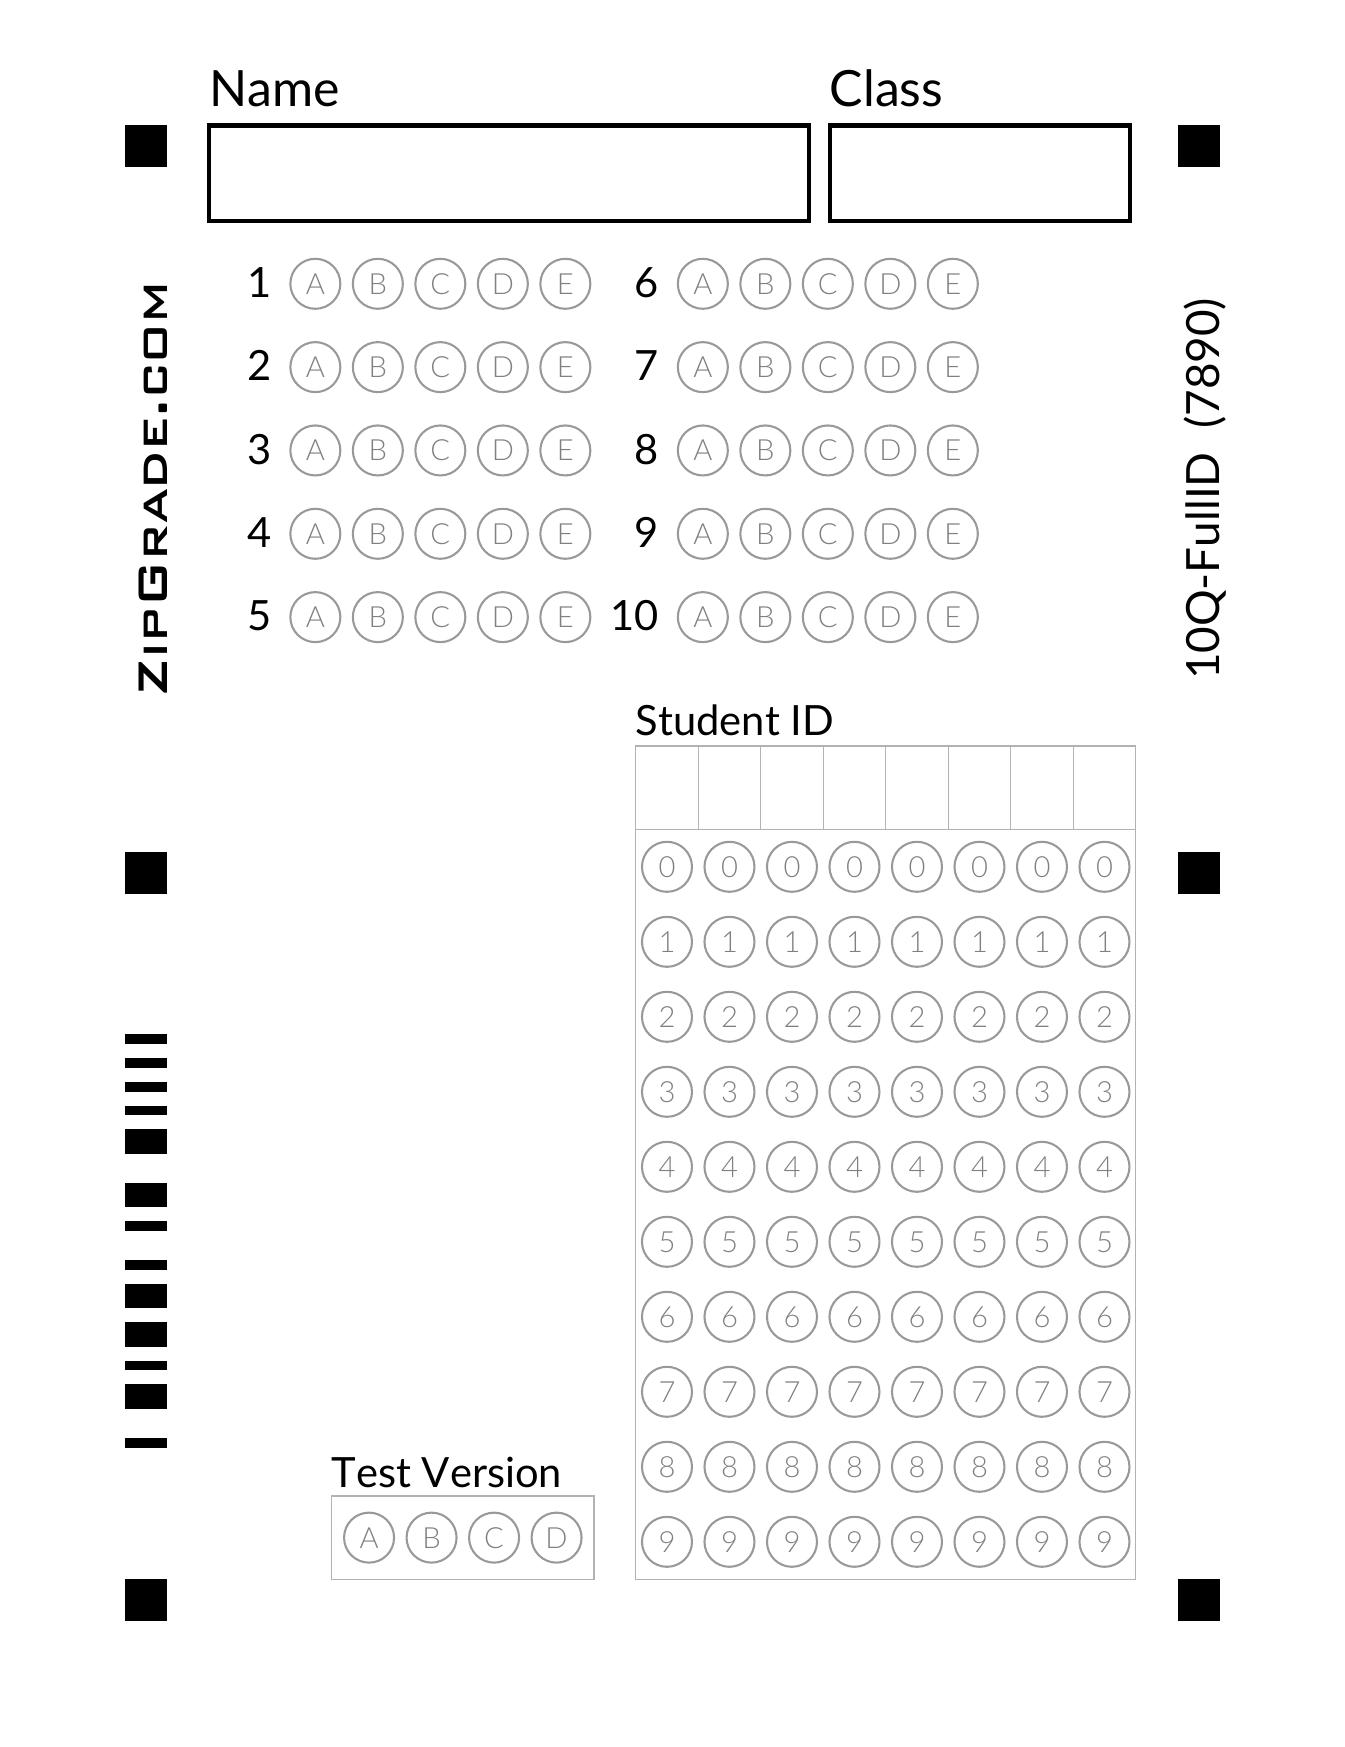
\includegraphics[height=5in]{7890.png}};
      \fill (#1,#2) circle (0.2);
    \end{tikzpicture}
  
    \bottommatter
  \end{flushright}
}



  \drawscantron{2.8}{1.65}
  \topmatter

\pagebreak

  \drawscantron{3.25}{1.65}
  \topmatter

\pagebreak

  \drawscantron{3.7}{1.65}
  \topmatter

\pagebreak

  \drawscantron{4.15}{1.65}
  \topmatter


\end{document}